\documentclass{standalone}
\usepackage{amsmath}
\usepackage{amssymb}
\usepackage{warpcol}
\usepackage{array}
\usepackage{esint}
\usepackage{subfig}
\usepackage{rotating}
\usepackage{booktabs}
\usepackage{paralist}
\usepackage{graphicx}
\usepackage{physics}
\usepackage{ucs}
\usepackage{indentfirst}
\usepackage{tikz}
\usepackage{colortbl}
\usepackage{xcolor}
\usepackage{xeCJK}
    \setCJKmainfont[BoldFont={Noto Serif CJK SC Bold},ItalicFont={FangSong}]{Noto Serif CJK SC}
    \setCJKsansfont[BoldFont={Noto Sans CJK SC Bold},ItalicFont={KaiTi}]{Noto Sans CJK SC}
    \setCJKmonofont[BoldFont={Noto Sans Mono CJK SC Bold}]{Noto Sans Mono CJK SC}

\DeclareUnicodeCharacter{"00B0}{\textdegree}
\DeclareUnicodeCharacter{"2103}{\textcelsius}

\pgfsetxvec{\pgfpoint{1.5em}{0}}
\pgfsetyvec{\pgfpoint{0}{1.5*1.732em}}

\usetikzlibrary{angles,patterns,datavisualization,plotmarks,arrows.meta,datavisualization.formats.functions,decorations.markings}

\newcommand{\hexagon}[2]{
    \draw[line cap=round] (#1,#2) -- (#1+1,#2) -- (#1+1.5,#2+.5) -- (#1+1,#2+1) -- (#1,#2+1) -- (#1-.5,#2+.5) -- (#1,#2);
}

\begin{document}
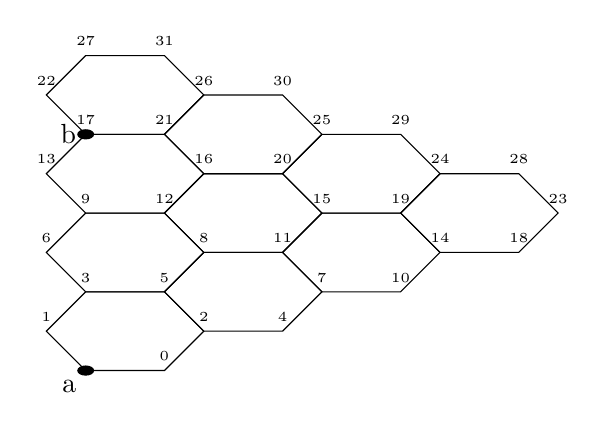
\begin{tikzpicture}
\foreach \x[evaluate=\x as \ymax using 3-\x/1.5,count=\xi] in {0,1.5,...,4.5}{
    \foreach \y in {0,...,\ymax}{
        \hexagon{\x}{\xi*.5-.5+\y}
    }
}
\foreach \x/\y[count=\idx] in {
    1/0, -.5/.5,
    1.5/.5, 0/1,
    2.5/.5, 1/1, -.5/1.5,
    3/1, 1.5/1.5, 0/2,
    4/1, 2.5/1.5, 1/2, -.5/2.5,
    4.5/1.5, 3/2, 1.5/2.5, 0/3,
    5.5/1.5, 4/2, 2.5/2.5, 1/3, -.5/3.5,
    6/2, 4.5/2.5, 3/3, 1.5/3.5, 0/4,
    5.5/2.5, 4/3, 2.5/3.5, 1/4
}{
    \node[above] at (\x, \y) {\tiny\pgfmathparse{int(\idx-1)}\pgfmathresult};
}
\filldraw (0, 0) node[below left] {a} ellipse (0.1 and 0.1/3^.5);
\filldraw (0, 3) node[left] {b} ellipse (0.1 and 0.1/3^.5);
\end{tikzpicture}
\end{document}
